\documentclass[tikz, border=5pt]{standalone}
\usetikzlibrary{calc, intersections}

\begin{document}
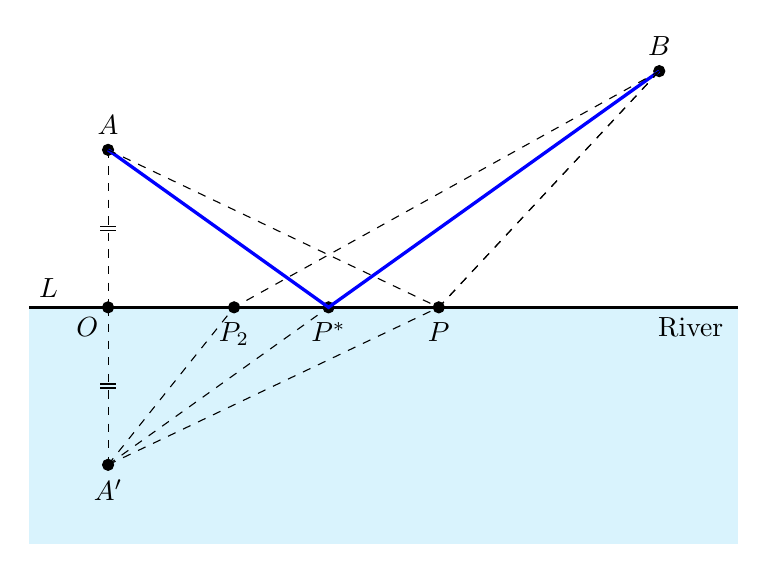
\begin{tikzpicture}
    %% Heron's problem

    % Params
    \def\xA{1}
    \def\yA{2}
    \def\xB{8}
    \def\yB{3}
    \def\xCp{5.2}
    \def\xCpp{2.6}

    % River y=0
    \fill[cyan!15] (\xA-1,0) rectangle (\xB+1,-\yA-1);
    \draw[very thick] (\xA-1,0) -- (\xB+1,0);
    \node at (\xB+0.4,0) [below] {River};

    % Coords
    \coordinate (A) at (\xA,\yA);
    \coordinate (B) at (\xB,\yB);
    \coordinate (O) at (\xA,0);  % Projection of A onto river
    \coordinate (Aprime) at (\xA,{-\yA});  % Reflection of A over river
    \coordinate (P) at (\xCp,0);
    \coordinate (P2) at (\xCpp,0);

    % Paths
    \path[name path=lineAB] (Aprime) -- (B);
    \path[name path=river] (\xA-1,0) -- (\xB+1,0);
    \path[name intersections={of=lineAB and river, by=Pstar}];

    % Points
    \draw[fill=black] (A) circle (2pt);
    \draw[fill=black] (B) circle (2pt);
    \draw[fill=black] (O) circle (2pt);
    \draw[fill=black] (Aprime) circle (2pt);
    \draw[fill=black] (Pstar) circle (2pt);
    \draw[fill=black] (P) circle (2pt);
    \draw[fill=black] (P2) circle (2pt);

    % Labels
    \node[above right] at (0,0) {\( L \)};
    \node[above=2pt] at (A) {\( A \)};
    \node[above=2pt] at (B) {\( B \)};
    \node[below left] at (O) {\( O \)};
    \node[below=2pt] at (Aprime) {\( A' \)};
    \node[below=2pt] at (Pstar) {\( P^* \)};
    \node[below=2pt] at (P) {\( P \)};
    \node[below=2pt] at (P2) {\( P_2 \)};

    % Segments
    \draw[dashed] (A) -- (O);
    \draw[dashed] (O) -- (Aprime);
    \draw[dashed] (Aprime) -- (B);
    \draw[very thick, blue] (A) -- (Pstar) -- (B);
    \draw[dashed] (Aprime) -- (P) -- (B);
    \draw[dashed] (A) -- (P) -- (B);
    \draw[dashed] (Aprime) -- (P2) -- (B);

    % Segment ticks
    \draw[line width=0.5pt] (\xA-0.1,0.975) -- (\xA+0.1,0.975);
    \draw[line width=0.5pt] (\xA-0.1,1.025) -- (\xA+0.1,1.025);
    \draw[line width=0.5pt] (\xA-0.1,-0.975) -- (\xA+0.1,-0.975);
    \draw[line width=0.5pt] (\xA-0.1,-1.025) -- (\xA+0.1,-1.025);

\end{tikzpicture}
\end{document}
